\chapter{Análise dos Resultados}
\label{cap:04}

Relatar os resultados obtidos a partir dos experimentos e dos estudos realizados. 


\section{Resultados/Impactos}

Resultados.


\section{Orçamento}

Orçamento, caso exista.


\section{Cronograma do Trabalho}

Segue abaixo o cronograma de trabalho das atividades realizadas e das que serão executadas até a Avaliação Final de TCC.

\textbf{Obs:} Para facilitar, crie o cronograma usando o modelo do Word contido no projeto (imagens/templateCronograma.docx), ou qualquer outro \textit{software}, salve a imagem e atualize o arquivo imagens/cronograma.png.

\FloatBarrier
\begin{figure*}[!htbp]
	\centering
	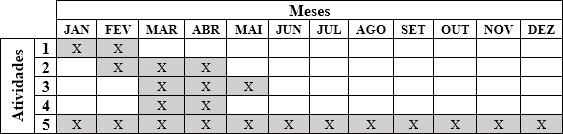
\includegraphics[scale=1]{imagens/cronograma}
\end{figure*}
\FloatBarrier

\begin{enumerate}
	\item Descrição da atividade 1;
	\item Descrição da atividade 2;
	\item Descrição da atividade 3;
	\item Descrição da atividade 4;
	\item Descrição da atividade 5.
\end{enumerate}
